\section{Frozen Development Results}

\begin{cautionbox}
\textbf{Provenance.} Every number in this section belongs to the frozen V2
artifact root and historical execution model. These are results of that
experiment, not estimates from the current simulator. V2 also applied REST
snapshot state at a pre-fetch local tag. The timing proxy audit does not prove
that its execution-derived values are invariant to the post-response-gated
exchange-clock policy.
\end{cautionbox}

\subsection{Phase A: passive baseline}

The fixed microprice maker was unprofitable in 18 of 24 windows at both queue
endpoints. Table \ref{tab:phase-a} reports window means and 95\% bootstrap
intervals. Proportional cancellation credit produced a wholly negative
interval. The no-credit interval crossed zero, but its point estimate was also
negative. No stable passive edge was demonstrated. This conclusion retains the
queue-model dependence of the uncertainty.

The fee hurdle is economically central. At a representative 71,500 USDT price,
the 2 USDT half-spread is about 0.28 bps per side, while the simulation charges
2 bps per maker fill. In the pooled fee diagnostic, completed matched lots would
break even at maker fees of \MatchedBreakEvenQcZero\ bps under no cancellation
credit and \MatchedBreakEvenQcOne\ bps under proportional credit. Including the
hourly residual-inventory marks, the full strategy would instead require maker
rebates of \FullRebateQcZero\ and \FullRebateQcOne\ bps,
respectively. The baseline is therefore a demanding execution diagnostic, not a
configuration with an assumed spread advantage over fees.

The frozen fee summary metadata calls this a ``window-close'' mark. That phrase
is a preserved wording error: the computation marks each one-hour session end
and resets state before the next session. The numeric rows are unchanged.

\begin{table}[H]
\centering
\caption{Frozen legacy Phase A full-strategy net P\&L per nominal five-hour
development window. Each row sums five independently initialized, hourly marked
episodes (0.001 BTC quotes, 0.01 BTC maximum position, 2 bps maker fee).}
\label{tab:phase-a}
\begin{tabular}{@{}lrrr@{}}
\toprule
Queue credit & Mean (USDT) & 95\% CI low & 95\% CI high \\
\midrule
0 (no credit) & \PhaseAQcZeroMean & \PhaseAQcZeroLow & \PhaseAQcZeroHigh \\
1 (proportional) & \PhaseAQcOneMean & \PhaseAQcOneLow & \PhaseAQcOneHigh \\
\bottomrule
\end{tabular}
\end{table}

The original reference was microprice because it can encode top-of-book
imbalance. Its own one-second signal was nevertheless weak: $+0.0190$ bps per
signal standard deviation, HAC $t=1.74$, with a positive coefficient in 19 of
24 windows. It missed both the $|t|\ge2$ and 0.05 bps materiality gates. This
motivated OFI as a richer event-flow signal without claiming that the baseline
was optimized out of trouble.

\subsection{Phase B: OFI population evidence}

Normalized OFI passed all three population gates. The one-second coefficient
was positive in 24 of 24 windows. Its unconditional bucket response rose
monotonically from $-0.276$ bps in the lowest bucket to $+0.284$ bps in the
highest. Table \ref{tab:ofi-regression} shows that statistical significance
persists at longer horizons while explanatory power falls sharply.

\begin{table}[H]
\centering
\caption{Frozen legacy pooled normalized-OFI regressions on forward mid drift.}
\label{tab:ofi-regression}
\begin{tabular}{@{}lrrrr@{}}
\toprule
Horizon & Observations & Slope & HAC $t$ & Effect / 1 s.d. (bps) \\
\midrule
1 s  & 430,278 & 0.1192 & 64.63 & 0.1233 \\
10 s & 430,062 & 0.2424 & 35.83 & 0.2507 \\
1 m  & 428,862 & 0.3157 & 18.06 & 0.3268 \\
5 m  & 423,102 & 0.2958 &  7.48 & 0.3069 \\
\bottomrule
\end{tabular}
\end{table}

The one-second regression $R^2$ is only \OFIRSquared. The large $t$-statistic
reflects a repeatable short-horizon association in a densely sampled series. It
does not imply that the signal explains most price variation or can be captured
after execution and costs.

\begin{figure}[H]
  \centering
  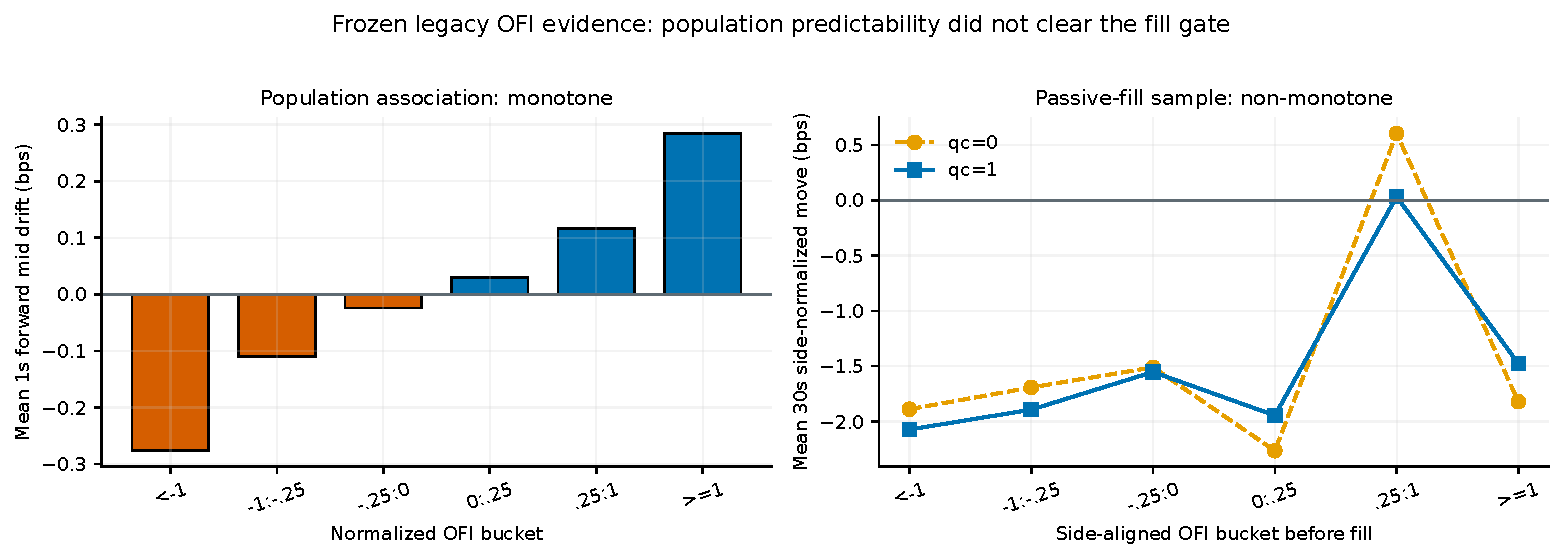
\includegraphics[width=0.98\textwidth]{figures/ofi_population_vs_fills.pdf}
  \caption{Unconditional and fill-conditioned OFI evidence. The left panel is
  queue-independent. The right panel uses historical baseline fills and must
  be interpreted under the legacy execution model.}
  \label{fig:ofi-population-fill}
\end{figure}

\subsection{Phase B: the conditional gate}

The pre-specified 30-second conditional comparison was only
\OFIConditionalQcOne\ bps at $c=1$ and \OFIConditionalQcZero\ bps at $c=0$,
far below 1.0 bps. Its selected bucket counts were respectively
\OFIMinCountQcOne\ and \OFIMinCountQcZero, exceeding the minimum-count rule.
The full response was not monotone. In particular, the smaller
$[0.25,1)$ bucket appeared more favorable than the selected adverse bucket at
both endpoints, but had only 71 and 54 observations. That is an exploratory
pattern, not a post-hoc replacement for the defined test and not a powered
estimate of a tradeable threshold.

The defensible result is consequently precise: the defined fill-conditioned
gate failed at both queue endpoints, and the broader bucket pattern was not
stable or monotone enough to advance the candidate. It would be too strong to
say that OFI's predictive content universally ``vanished'' on fills, or that an
unrun \code{OFIGatedMM} necessarily loses.

\subsection{Phase C: queue and latency stress}

At 10 ms entry latency, granting more cancellation credit raised modeled fill
throughput but worsened both quantity-weighted matched-lot economics and total
strategy P\&L. This monotone economic deterioration is stronger evidence than
the sign flip observed in the earlier six-anchor analysis.

\begin{table}[H]
\centering
\caption{Frozen legacy pooled Phase C results at 10 ms. ``Orders/fill'' is a throughput
diagnostic, matched net/BTC weights pooled matched quantity.}
\label{tab:queue-stress}
\begin{tabular}{@{}rrrrr@{}}
\toprule
Credit & Fills & Orders/fill & Matched net/BTC & Full net P\&L \\
\midrule
0.00 & 1,595 & 70.8 &  $-9.75$ & $-16.46$ \\
0.25 & 1,796 & 62.9 & $-15.08$ & $-17.64$ \\
0.50 & 1,802 & 62.6 & $-16.08$ & $-20.88$ \\
0.75 & 1,831 & 61.6 & $-17.51$ & $-21.33$ \\
1.00 & 2,041 & 55.4 & $-23.65$ & $-25.03$ \\
\bottomrule
\end{tabular}
\end{table}

\begin{figure}[H]
  \centering
  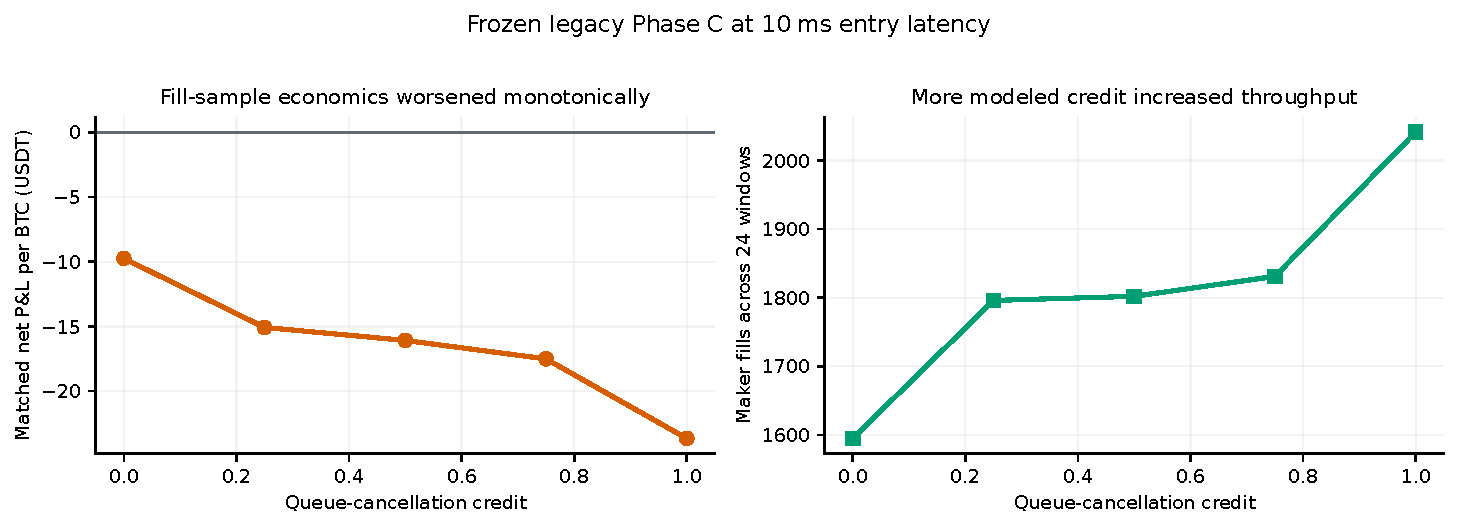
\includegraphics[width=0.92\textwidth]{figures/queue_credit_stress.pdf}
  \caption{Queue-credit sensitivity. More favorable modeled queue advancement
  selects a larger pooled fill sample with worse mean matched economics. The
  sweep does not establish that fill sets are nested.}
  \label{fig:queue-stress}
\end{figure}

The historical $0/10/50$ ms entry-latency sweep was numerically unchanged at
the two credit endpoints. Under \LegacyModel, order eligibility was quantized
to the next depth update, so this is evidence about a model limitation rather
than evidence that real latency is irrelevant. It was one reason to build the
event-driven clock.

\subsection{Tails and bounded replay audits}

Under proportional credit, the worst 5\% of 30-second fill observations
accounted for 40.64\% of the summed adverse movement. The worst 5\% of matched
lots accounted for 86.62\% of total matched-lot loss. Fill toxicity was thus
broad with meaningful tails, whereas realized matched-lot loss was far more
tail-concentrated. These ratios depend on the signed-total denominator and are
reported with negative-only denominators in the artifacts as well.

The panel-wide same-millisecond audit found 10 overlap fills among 2,041 fills
at $c=1$ (0.49\%) and 7 among 1,595 at $c=0$ (0.44\%). It found zero
\emph{artifact-evidenced} contradictions of the depth-before-trade assumption.
That bounded label matters: reconciliation artifacts do not persist every
queue-drain timestamp, so candidate rows cannot all be adjudicated after the
fact. Separately, all six original anchor windows were aggregate-trade-gap
clean, and replaying them under the later fail-closed trade-gap policy changed
no reported value.

\subsection{Decision}

No strategy advanced. The baseline did not demonstrate stable positive
economics, microprice was weak, and OFI cleared the population screen but not
the specified execution-conditioned premise. Phase C showed that reasonable
variation in unobserved queue advancement changed throughput and loss magnitude
without producing positive pooled matched economics. No candidate strategy was
evaluated on the holdout. This is a negative/conditional development result,
not a live-performance claim.
